% This is LLNCS.DEM the demonstration file of
% the LaTeX macro package from Springer-Verlag
% for Lecture Notes in Computer Science,
% version 2.4 for LaTeX2e as of 16. April 2010
%
\documentclass{llncs}
\pagestyle{plain}  % switches on printing of running heads
%
\usepackage{makeidx}  % allows for indexgeneration
\usepackage{graphicx}
\usepackage{pgf}
\usepackage{tikz}
\usepackage{wasysym}
\usepackage{listings}
\usepackage[]{algorithm2e}

\usetikzlibrary{arrows,automata,positioning}

%
\begin{document}
%
\frontmatter          % for the preliminaries
%

\begin{titlepage}
	
\vspace*{4cm}

\begin{center} 
	
\textsc{\LARGE University of Bayreuth}\\[1.5cm]

\textsc{\LARGE Bachelor Seminar Tree Automata}\\[0.5cm]

% Title
\newcommand{\HRule}{\rule{\linewidth}{0.5mm}}
\HRule \\[0.4cm]
{	\huge \bfseries Introduction to Ranked Tree Automata\\[0.4cm] }
\HRule \\[1.5cm]

% Author and supervisor
\begin{minipage}{0.4\textwidth}
	\begin{flushleft} \large
		\emph{Author:}\\
		Martin \textsc{Braun}
	\end{flushleft}
\end{minipage}
\hfill
\begin{minipage}{0.4\textwidth}
	\begin{flushright} \large
		\emph{Supervisor:} \\
		Prof. Dr. Wim \textsc{Martens}
	\end{flushright}
\end{minipage}

\end{center}

\end{titlepage}

\newcommand{\nfaExample}{
	 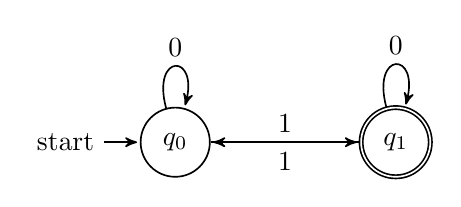
\begin{tikzpicture}[->,>=stealth',shorten >=1pt,auto,node distance=2.8cm,
                 		   semithick]
 				\tikzstyle{every state}=[fill=white,draw=black,text=black]
		
				\node[initial,state]		(A)			{$q_0$};
				\node[state,accepting]	(B)	[right of=A]	{$q_1$};
	
 				 \path (A)	edge	[loop above]	node {0}	(A)
					(A)	edge			node {1}	(B)
					(B)	edge	[loop above]	node {0}	(B)
					(B)	edge			node {1}	(A);
	\end{tikzpicture}
}

\newcommand{\moveStar}{\rightarrow_A^*}
\newcommand{\moveStarDet}{\rightarrow_{A_d}^*}

\newcommand{\simpleTreeExample} {
	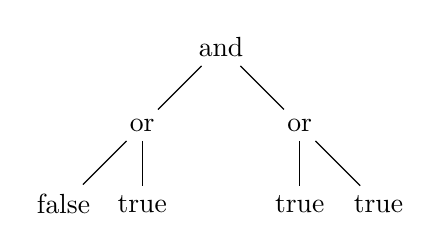
\begin{tikzpicture}[auto]
	\node (and) at (2, 3) {and};
	\node (or1) at (1, 2) {or};
	\node (or2) at (3, 2) {or};
	\node (false1) at (0, 1) {false};
	\node (true1) at (1, 1) {true};
	\node (true2) at (3, 1) {true};
	\node (true3) at (4, 1) {true};
	
	\draw [-] (and) to (or1);
	\draw [-] (and) to (or2);
	\draw [-] (or1) to (false1);
	\draw [-] (or1) to (true1);
	\draw [-] (or2) to (true2);
	\draw [-] (or2) to (true3);
	\end{tikzpicture}
}


\chapter*{Introduction to Tree Languages}
A good example for a tree language is the one consisting of boolean expressions for which an instance - if formatted in the right way - could look like this:

\begin{center}
	\(and(or(false, true), or(true, true))\)\\
\end{center}
In order to ease understanding, the elements of the language are often represented as a tree in a graphical way:
\begin{center}
	\simpleTreeExample
\end{center}
~\\
Just like for "normal" regular languages, it is of interest to know whether a given word (in this case a tree) is part of the (tree-)language. In order to describe an automaton that recognizes tree-languages we have to define what \textbf{\(\Sigma\)-trees} and (regular) \textbf{tree-languages} are, first.

\begin{definition}{\(\Sigma\)-tree \cite{automata-xml}}
	\\
	The set of \(\Sigma\)-trees \(T_\Sigma\) over the alphabet \(\Sigma\) is inductively defined as follows:
	\begin{center}
		1. every \(\sigma \in \Sigma\) is a \(\Sigma\)-tree\\
		2. \(\sigma \in T_\Sigma\) and \(t_1,...,t_n \in T_\Sigma, n \ge 1 \iff \sigma(t_1,...,t_n) \in T_\Sigma\) 
	\end{center}
\end{definition}
~\\
\textit{Note: Normally, there is no bound for the number of children in a tree (these trees are called \textit{unranked}), but in this draft we will only take a look at \textbf{ranked trees}, which have such a bound.}

\begin{definition}{tree-language \cite{automata-xml}}
	\\
	A tree language \(L_{t\Sigma}\) over the alphabet \(\Sigma\) is defined as a subset of \(T_\Sigma\):
	\begin{center}
		\(L_{t\Sigma} \subseteq T_\Sigma\)
	\end{center}
	\(\Rightarrow T_\Sigma\) is already a tree-language.	
\end{definition}

Next, we have to declare some special words in the context of $\Sigma-trees$.

\begin{definition}{variables, linear terms, ground-terms} \cite{tata-nfta}\cite{wiki-groundterm}\\
	Let \(v \notin \Sigma = \emptyset\) be a constant (symbol with no child). We call $v$ a \textbf{variable} in a term over the ranked alphabet \(\Sigma\) if it is a placeholder
	for any given \(\sigma \in \Sigma\) in that term. Terms containing every $v$ at most once are \textbf{linear terms}. All terms that don't contain any variables, are called \textbf{ground-terms} over \(\Sigma\).\\
\end{definition}

\pagebreak
We can now define (Non-Deterministic) Finite Tree Automata for tree languages.
\\
\\
\textit{Note: this definition will be expanded with more terms later in this draft and some of the content in this definition will get a specific name assigned to them. But in order to not overcomplicate the definition, these parts are left out for now.}

\begin{definition}{NFTA \cite{tata-nfta}}
	\\
	A (Non-Deterministic) Finite Tree Automaton (NFTA) over the \textbf{alphabet \(\Sigma\)} is a tuple \(A = (Q, \Sigma, Q_f ,\Delta)\) where
	\(Q\) is a \textbf{finite set of states}, \(Q_f \subseteq Q\) is a  \textbf{finite set of final states}, and \(\Delta\) is a \textbf{finite set of transition rules} of the type:
	
	\begin{center}
		\(f(q_1,...,q_n) \rightarrow q_x\) \\
		where \(n \ge 0, f \in \Sigma, q_x, q_1,...,q_n \in Q \)
	\end{center}
	For \(n = 0\), we write:
	\begin{center}
		\(a \rightarrow q(a)\) \\
		where  \(a \in \Sigma, q \in Q \)
	\end{center}
	~\\
	Tree automata over \(\Sigma\) run on ground terms over \(\Sigma\). An automaton starts at
	the leaves and moves upward, associating along a \textbf{run} a state with each subterm
	inductively while reducing the tree via the transition rules.
	\\\\
	For a tree $t' \in T_{\Sigma \cup Q}$ that is the result of applying a transition rule on a tree $t \in T_{\Sigma \cup Q}$ we write:
		$$t \rightarrow_A t'$$
	If more or equal than one transition rules are applied we denote it like this:
		$$t \moveStar t'$$	
	$\moveStar$ is the reflexive and transitive closure of $\rightarrow_A$.\\
\end{definition}
\textit{
	Note: There is no initial state in an NFTA but the ground-terms (which can be considered to be the "initial rules" of the NFTA) act alike by transitioning constant symbols into a state.
}
\\

\pagebreak

Our binary-boolean-expression NFTA can now be written as:

\begin{example}{binary-boolean-statement NFTA}
	\\
	\(A = (Q, \Sigma, Q_f ,\Delta)\)
	\newline
	\(\Sigma = \{or, and, not, true,false\}\)
	\newline
	\(Q = \{q_f,q_t\}\)
	\newline
	\(Q_f = \{q_t\}\)
	\newline
	\(\Delta = \{ false \rightarrow q_f, true \rightarrow q_t,
	\newline
	~~~~~~~~~and(q_t, q_t) \rightarrow q_t, and(q_t, q_f) \rightarrow q_f, and(q_f, q_t) \rightarrow q_f, and(q_f, q_f) \rightarrow q_f,
	\newline
	~~~~~~~~~or(q_t,q_t) \rightarrow q_t, or(q_t, q_f) \rightarrow q_t, or(q_f, q_t) \rightarrow q_t, or(q_f, q_f) \rightarrow q_f,
	\newline
	~~~~~~~~~not(q_f) \rightarrow q_t, not(q_t) \rightarrow q_f\}\)
\end{example}

A run with the example input from the beginning of this chapter looks like this:

\begin{example}{running a NFTA}
\\
\begin{table}
	\centering
	\begin{tabular}{c c}
		\simpleTreeExample
		&
		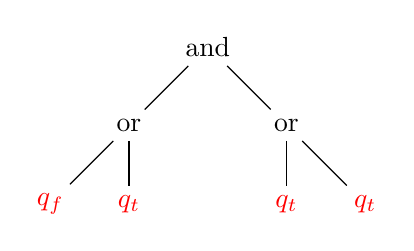
\begin{tikzpicture}[auto]
			\node (and) at (2, 3) {and};
			\node (or1) at (1, 2) {or};
			\node (or2) at (3, 2) {or};
			\node (false1) at (0, 1) {\textcolor{red}{$q_f$}};
			\node (true1) at (1, 1) {\textcolor{red}{$q_t$}};
			\node (true2) at (3, 1) {\textcolor{red}{$q_t$}};
			\node (true3) at (4, 1) {\textcolor{red}{$q_t$}};
			
			\draw [-] (and) to (or1);
			\draw [-] (and) to (or2);
			\draw [-] (or1) to (false1);
			\draw [-] (or1) to (true1);
			\draw [-] (or2) to (true2);
			\draw [-] (or2) to (true3);
		\end{tikzpicture}
		\\
		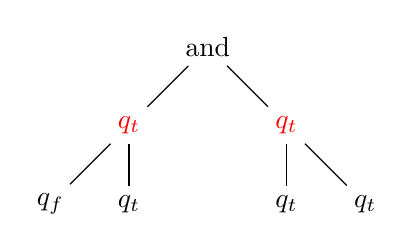
\begin{tikzpicture}[auto]
		\node (and) at (2, 3) {and};
		\node (or1) at (1, 2) {\textcolor{red}{$q_t$}};
		\node (or2) at (3, 2) {\textcolor{red}{$q_t$}};
		\node (false1) at (0, 1) {$q_f$};
		\node (true1) at (1, 1) {$q_t$};
		\node (true2) at (3, 1) {$q_t$};
		\node (true3) at (4, 1) {$q_t$};
		
		\draw [-] (and) to (or1);
		\draw [-] (and) to (or2);
		\draw [-] (or1) to (false1);
		\draw [-] (or1) to (true1);
		\draw [-] (or2) to (true2);
		\draw [-] (or2) to (true3);
		\end{tikzpicture}
		&
		\begin{tikzpicture}[auto]
		\node (and) at (2, 3) {\textcolor{red}{$q_t$}};
		\node (or1) at (1, 2) {$q_t$};
		\node (or2) at (3, 2) {$q_t$};
		\node (false1) at (0, 1) {$q_f$};
		\node (true1) at (1, 1) {$q_t$};
		\node (true2) at (3, 1) {$q_t$};
		\node (true3) at (4, 1) {$q_t$};
		
		\draw [-] (and) to (or1);
		\draw [-] (and) to (or2);
		\draw [-] (or1) to (false1);
		\draw [-] (or1) to (true1);
		\draw [-] (or2) to (true2);
		\draw [-] (or2) to (true3);
		\end{tikzpicture}
		\\
		\begin{tikzpicture}[auto]
		\node (and) at (2, 3) {$q_t$};
		\node (or1) at (1, 2) {$q_t$};
		\node (or2) at (3, 2) {$q_t$};
		\node (false1) at (0, 1) {$q_f$};
		\node (true1) at (1, 1) {$q_t$};
		\node (true2) at (3, 1) {$q_t$};
		\node (true3) at (4, 1) {$q_t$};
		
		\draw [-] (and) to (or1);
		\draw [-] (and) to (or2);
		\draw [-] (or1) to (false1);
		\draw [-] (or1) to (true1);
		\draw [-] (or2) to (true2);
		\draw [-] (or2) to (true3);
		\end{tikzpicture}
		&
		done.
	\end{tabular}
\end{table}
\\
Or in written form:\\
\(and(or(false, true), or(true, true)) \moveStar and(or(q_f, q_t), or(q_t, q_t)) \\ \moveStar and(q_t, q_t) \moveStar q_t \)\\\\
\(q_t \in Q_f \Rightarrow\) A accepts w \(\Rightarrow w \in L_A \) with \(L_A\) being the language recognized by the automaton.
\\
\\
\end{example}

\chapter*{Determinization}

Non Deterministic Finite Tree Automata (NFTA) can be determinized just like Non Determinitistic Automata (NFA) in the word case. By knowing that there exists a DFTA for every NFTA, some algorithms become easier to write and proof. We will now take a look at how this is done. But first we have to define formally, what being deterministic means in the context of FTAs.

\begin{definition}{Deterministic Finite Tree Automaton}

	A tree automaton with no two rule of the type:
	\begin{center}
		\(f(q_1,..., q_n) \rightarrow q_x\)\\
		\(f(q_1,...,q_n) \rightarrow q_y\)\\
		(Note: this includes the ground-terms)
	\end{center}
	or
	\begin{center}
		\(\epsilon(q_1, ..., q_n) \rightarrow q_x\)
	\end{center}
	with \(n \ge 0, q_x,q_y,q_1,...q_n \in Q, q_x \neq q_y, a \in \Sigma\)
	is called a \textbf{Deterministic Finite Tree Automaton} (DFTA).
\end{definition}

Similar to the algorithm for Determinization in the word case, there exists a power set construction algorithm for determizing Tree Automata.

\begin{definition}{\textbf{Algorithm DET} for Tree Automata \cite{tata-nfta}}
\\
\begin{algorithm}[H]
	\KwData{NFTA \(A = (Q, \Sigma, Q_f ,\Delta)\)}
	\(Q_d := \emptyset\)\\
	\(\Delta_d := \emptyset\)
	\\
		\While{\(\Delta_d\) grew last cycle} {
			\( f(q_1,...,q_n) \in \Delta\)\\
			\(s_1,...,s_n \in Q_d\)\\
			/* meta-state representing the set of reachable states */ \\
			\( s := state(\{ q \in Q ~|~ \exists q_1 \in s_1,..., q_n \in s_n, f(q_1,...q_n) \rightarrow q \in \Delta \}) \)\\~\\
			\(Q_d := Q_d \cup \{s\}\)\\
			\(\Delta_d := \Delta_d \cup f(s_1,...,s_n) \rightarrow s \)
		}
	\(Q_{f_d} := \{ s \in Q_d ~ | ~ \{s\} \cap Q_d \neq \emptyset \}\)\\
	\KwResult{DFTA \(A_d = (Q_d, \Sigma, Q_{f_d}, \Delta_d) \)}
\end{algorithm}
\end{definition}

It is easy to see, that the algorithm produces a deterministic automaton \(A_d\) as we are automatically constructing meta-states for all reachable states and therefor eliminating all possible non-deterministic behaviour.

\pagebreak

However, we still have to prove that \(L(A) = L(A_d)\).\newline 
For this, we have to show that the meta-states \(s \in Q_d\) are "built correctly", or in formal terms:

\begin{center}
	\(For~any~tree~t: t \moveStarDet s \iff s = state(\{q \in Q ~|~ t \moveStar q\})\)
\end{center}


\begin{proof}{\(L(A) = L(A_d)\) (Correctness of DET) \cite{tata-nfta}}\\
	This proof is done via an induction over the structure of the symbols in \(\Sigma\).
	\begin{itemize}
		\item \textbf{Base case:}
			For any tree \(t = a \in \Sigma\) we take a look at the corresponding ground-term \(a \rightarrow q(a)\). Because of the way we defined \(s\) as the meta-state representing the set of all reachable states in a given situation this is inherently correct.
			\\
		\item \textbf{induction step: \(t = f(q_1,... , q_n)\)}
			\begin{itemize}
				\item 
				1.: \(t \moveStarDet s \Rightarrow (s = state(\{q \in Q ~|~ t \moveStar q\})\)\\\\
				Supposing \(t \moveStarDet f(s_1, ..., s_n) \rightarrow_{A_d} s\), by induction hypothesis, for each \(i \in {1,..., n}\), we can see that \(s_i = state(\{q \in Q ~|~ q_i \moveStar q\}\).\\
				\\
				Since states \(s_i \in Q_d\), rules \(f(s_1, ..., s_n) \rightarrow s \in \Delta_d\) are added by the determinization algorithm and \( s := state(\{ q \in Q ~|~ \exists q_1 \in s_1,..., q_n \in s_n, f(q_1,...q_n) \rightarrow q \in \Delta \}) \), we can see that	\(s = state(\{q \in Q ~|~ t \moveStar q\})\).
				\\
				\item
				2.: \(s = state(\{q \in Q ~|~ t \moveStar q\}) \Rightarrow t \moveStarDet s\)\\\\
				Considering \(s = state(\{q \in Q ~|~ f(q_1, ..., q_n) \moveStar q\})\) with state sets \(S_i\) defined as \(S_i := \{q \in Q ~|~ q_i \moveStar q\}\), by induction hypothesis for each \(i \in \{1, ..., n\}\) we know \(q_i \moveStarDet s_i = state(S_i)\).
				Thus \( s := state(\{ q \in Q ~|~ \exists q_1 \in s_1,..., q_n \in s_n, f(q_1,...q_n) \rightarrow q \in \Delta \}) \).\\
				\\
				By the definition of \(\Delta_d\) in the determinization algorithm, \(f(s_1, ..., s_n) \in \Delta_d\) and thus \(t \moveStarDet s\).
			\end{itemize}
	\end{itemize}
	
\end{proof}

\pagebreak

\newcommand{\automatonDefinition} {
	\(A = (Q, \Sigma, Q_f, \Delta)\)
}

Following is an example of how a NFTA can be determinized with this algorithm.

	\begin{example}{Running the DET algorithm}
		\\
		consider an obviously non deterministic FTA given like this:\\
		\automatonDefinition\\
		\(\Sigma = \{ul, li, text, empty\}\)\\
		\(Q = \{q_{ul}, q_{li1}, q_{li2}, q_{text}, q_{empty}\}\)\\
		\(Q_f = \{q_{ul}\}\)\\
		\(\Delta = \{
		ul(q_{li1},q_{li2}) \rightarrow q_{ul}, ul(q_{li2},q_{li1}) \rightarrow q_{ul}, \newline
		li(q_{text},q_{text}) \rightarrow q_{li1}, li(q_{text}, q_{text}) \rightarrow q_{li2}\newline
		text \rightarrow q_{text}, empty \rightarrow q_{empty}, \newline
		\epsilon(q_{empty}) \rightarrow q_{text}
		\}\)
		\\\\
		This recognizes all trees that represent unordered lists (ul) in HTML notation that contain 2 list items (li) that are either empty or contain text:
			%careful: space indentation
			\lstset{
				basicstyle=\footnotesize, frame=tb,
				xleftmargin=.4\textwidth, xrightmargin=.5\textwidth
			}
			\begin{lstlisting}[frame=none]
<ul>
    <li>text</li>
    <li>empty</li>
</ul>
			\end{lstlisting}
			Or as a tree input:
			\begin{center}
				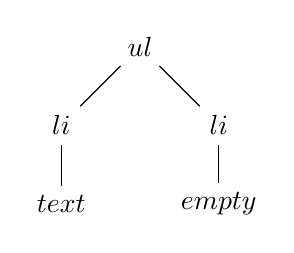
\begin{tikzpicture}[auto]
				\node (and) at (2, 3) {$ul$};
				\node (or1) at (1, 2) {$li$};
				\node (or2) at (3, 2) {$li$};
				\node (true1) at (1, 1) {$text$};
				\node (true2) at (3, 1) {$empty$};
				
				\draw [-] (and) to (or1);
				\draw [-] (and) to (or2);
				\draw [-] (or1) to (true1);
				\draw [-] (or2) to (true2);
				\end{tikzpicture}
			\end{center}
					If we start determinizing with the ground terms and then go "up in the hierarchy", we get these new rules and states:
					\\
					\(
					\newline
					text \rightarrow state(\{q_{text}\})
					\newline
					empty \rightarrow state(\{q_{text}, q_{empty}\})
					\newline
					li(state(\{q_{text}\}), state(\{q_{text}\})) \rightarrow state(\{q_{li1}, q_{li2}\})
					\newline
					li(state(\{q_{text}, q_{empty}\}), state(\{q_{text}, q_{empty}\})) \rightarrow state(\{q_{li1}, q_{li2}\})
					\newline
					ul(state(\{q_{li1}, q_{li2}\}), state(\{q_{li1}, q_{li2}\})) \rightarrow state(\{q_{ul}\})
					\)
					\\
					\\
				    And the set of final states is \(Q_{f_d} = \{state(\{q_{ul}\})\}\).
			\end{example}

\pagebreak

\chapter*{Minimization}

\begin{definition}{Context}\\
	A context $C \in C(\Sigma)$ is a tree 
\end{definition}

\pagebreak

%
% ---- Bibliography ----
%
\begin{thebibliography}{99}
%
\bibitem {automata-xml}
	Automata theory for XML researchers
	Frank Neven
	University of Limburg
	frank, neven~luc, ac. be,
	http://homepages.inf.ed.ac.uk/libkin/dbtheory/frank.pdf, 03/11/2015
\bibitem {tata-nfta}
	Tree Automata and Techniques, Hubert Comon et. al, Pages 19-39
\bibitem {wiki-groundterm}
	\url{http://en.wikipedia.org/wiki/Ground\_expression}, 03/16/2015




\end{thebibliography}

\end{document}
